%%%%%%%%%%%%%%%%%%%%%%%%%%%
% PREAMBOLO DEL DOCUMENTO %
%%%%%%%%%%%%%%%%%%%%%%%%%%%
\documentclass[a4paper,11pt,oneside,top=3cm,bottom=3cm,left=3.5cm,right=3.5cm,openright,reqno,table]{book}

% openany - fa iniziare i capitoli direttamente nella pagina successiva
% openright - fa iniziare i capitoli nella prima pagina destra disponibile 
% fleqn  - allinea le formule a sinistra anzichè centrarle
% leqno - dispone la numerazione delle formule sulla sinistra o destra
% reqno - dispone la numerazione delle formule sulla destra
%
\usepackage{packages}
% Per non appesantire troppo questo file
% quasi tutti i pacchetti usati sono salvati in packages.sty
%
\linespread{1.5}
% Per avere la parola BOZZA scritta su tutte le pagine

% funziona solo in modalità PS
% Invece per i PDF ho risolto così:
% pdftk tesi.pdf background bozza.pdf output tesi_bozza.pdf
%
%%%%%%%%%%%%%%%%%%%%%%%%%%%%%%%%%
%   DOCUMENTO VERO E PROPRIO    %
%%%%%%%%%%%%%%%%%%%%%%%%%%%%%%%%%
\begin{document}
% FRONTESPIZIO %
\begin{titlepage}
\changepage{}{}{}{-7.5 mm}{}{}{}{}{}
% parametri per cambiare le dimensioni di una singola pagina in ordine:
% {textheight}{textwidth}{evensidemargin}{oddsidemargin}{columnsep}
% {topmargin}{headheight}{headsep}{footskip}
% se voglio centrare la pagina devo mettere bindingoffset/2
% i primi 5 parametri posso usarli con \changetext


\begin{center}

\includegraphics [width=.15\columnwidth, angle=0]{unisa}\\ % height
\vspace{0.5cm}
{\LARGE \scshape Università degli Studi di Salerno}\\
\vspace{0.5cm}
{\Large Dipartimento di Informatica}\\
\vspace{0.1cm}
{\large Corso di Laurea Triennale in Informatica}\\
\vspace{1.5cm}
{\Large \scshape Tesi di Laurea} \\
\vspace{4cm}
{\Huge \bfseries Dalla $\alpha$lfa alla $\beta$eta } \\
\vspace{5cm}

\begin{minipage}[t]{7cm}
\flushleft
\textsc{Relatore}

Prof. \textbf{Fabio Palomba} \\
{\small Università degli studi di Salerno} \\[0.25cm]
\end{minipage}
\hfill
\begin{minipage}[t]{7cm}
\flushright
\textsc{Candidato}

\textbf{Giuseppe Pagano} \\
Matricola: 0512106337
\end{minipage}

\vspace{3cm}

%& & \\
%& Candidato & \\
%& \textbf{Fabiano Pecorelli} & \\
{\small Anno Accademico 2021-2022} %\\
%
%
\begin{comment}
\begin{table}[!h]
\centering
\begin{tabular}{c c c} %p{5cm}c
& Tesi di laurea & \\
& \textbf{Fabiano Pecorelli} & \\
& & \\[0.25cm]
Relatore \\
prof. \textbf{Andrea De Lucia} \\
{\small Università degli studi di Salerno} & & {\small Provincia di Salerno}\\
& & \\[0.5cm]
& {\small A.A. 2015-2016} & \\
\end{tabular}
\end{table}
\end{comment}
%
%
\end{center}

\end{titlepage}
%

\frontmatter
% quello che segue è in numerazione romana e i capitoli non verranno numerati
% se non si vuole che compaia il numero di pagina basta usare il comando:
%\nonumber

% RINGRAZIAMENTI %
\begin{titlepage}

\nonumber
\null \vspace {\stretch{1}}
	\begin{flushright}
%	\begin{verse}
\textit{INSERIRE QUI UNA DEDICA O UNA CITAZIONE} \\[5mm]
%	\end{verse}
	\end{flushright}



\end{titlepage}
% SOMMARIO %
\cleardoublepage
%\selectlanguage{italian}
\begin{abstract}

INSERIRE ABSTRACT
\\[1cm]
Gli scacchi sono da sempre un gioco tanto affascinante quanto complesso, ed è proprio questo li rende un terreno fertile per l'introduzione tecniche innovative di ricerca e valutazione. All'interno di questa tesi vengono affrontati gli algoritmi
più noti e vengono discusse le idee alla base della loro efficacia per infine accennare allo stato dell'arte del mondo dei motori scacchistici. In particolare vengono affrontati i concetti di mini-max e potatura alfa-beta, comuni alla quasi 
totalità degli algoritmi che tentano di risolvere giochi a turni quali scacchi e dama, e migliorie apportabili alla alfa-beta, applicate nel contesto degli scacchi computazionali ma generalizzabili 
per funzionare in un qualsiasi algoritmo mini-max (come NegaScout) o specifiche per il mondo degli scacchi computazionali e viene fornita un'idea generale su come costruire una funzione di valutazione adatta al gioco degli scacchi.
\end{abstract} 
% INDICI %
\phantomsection
\addcontentsline{toc}{chapter}{Indice}
\tableofcontents
% Il simbolo * serve per evitare che comapaia nell'indice
\clearpage
%\listoffigures
%\clearpage
%\listoftables
% GLOSSARIO
%\cleardoublepage
\phantomsection
\addcontentsline{toc}{chapter}{Glossario}
% per inserire l'elenco dei simboli e degli acronimi nell'indice
\printglossary
% Per stampare il glossario
% per aggiornarlo si deve eseguire da terminale:
% makeindex -s myDoc.ist -t myDoc.alg -o myDoc.acr myDoc.acn
% per inserire una voce nell'elenco:
% \newglossaryentry{voce_etichetta}{name={voce}, description={descrizione}}
% se non compare direttamente nel testo va inizializzata con:
% \glsadd{voce_etichetta}
% oppure se viene richiamata all'interno del testo:
% \gls{voce_etichetta}
% SIMBOLI E NOTAZIONI %
\cleardoublepage
\phantomsection
\addcontentsline{toc}{chapter}{Elenco delle figure}
% per inserire l'elenco dei simboli e degli acronimi nell'indice
%\printglossary[type=\acronymtype,title=Elenco delle figure]
% Per stampare l'elenco dei simboli
\listoffigures
\cleardoublepage
\phantomsection
\addcontentsline{toc}{chapter}{Elenco delle tabelle}
% per inserire l'elenco dei simboli e degli acronimi nell'indice
%\printglossary[type=\acronymtype,title=Elenco delle figure]
% Per stampare l'elenco dei simboli
\listoftables
% per aggiornarlo si deve eseguire da terminale:
% makeindex -s myDoc.ist -t myDoc.glg -o myDoc.gls myDoc.glo
% per inserire una voce nell'elenco:
% \newglossaryentry{voce_etichetta}{name={voce}, description={descrizione}}
% se non compare direttamente nel testo va inizializzata con:
% \glsadd{voce_etichetta}
% oppure se viene richiamata all'interno del testo:
% \gls{voce_etichetta}

\mainmatter
% quello che segue sarà in numerazione araba e i capitoli verranno numerati
%\part{Studio iniziale}
% CAPITOLI
\phantomsection
%\addcontentsline{toc}{chapter}{Introduzione}
\chapter{Introduzione}
\markboth{Introduzione}{}
% [titolo ridotto se non ci dovesse stare] {completo}

\section{Contesto applicativo} %\label{1sec:scopo}
Gli scacchi sono un gioco di strategia deterministico\footnote{Si definisce deterministico un gioco in cui gli stati assunti durante la partita sono determinati
unicamente dalle azioni dei giocatori, si parla quindi di giochi in cui non vi è una componente aleatoria.} a somma zero\footnote{Si definisce a somma zero un gioco in cui il guadagno o la perdita di un partecipante è perfettamente bilanciato da una perdita o un guadagno di un altro partecipante in una somma uguale e opposta.} e ad informazione completa\footnote{Si definisce ad informazione completa un gioco i cui stati sono
completamente espliciti ai giocatori, si parla quindi di giochi dove entrambi i giocatori hanno accesso a tutte le informazioni riguardanti lo stato della partita, non vi sono quindi "carte coperte" o elementi di sorpresa.}  
che si svolge su una tavola quadrata formata da 64 caselle, di due colori alternati,
detta scacchiera, sulla quale ogni giocatore contraddistinto da uno dei due colori (bianco o nero), dispone di 16 pezzi: un re, una regina, due alfieri, due cavalli, due torri e otto pedoni.
L'obiettivo del gioco è dare scacco matto, ovvero minacciare la cattura del re avversario mentre esso non
ha modo di rimuovere il re dalla sua posizione di pericolo alla sua prossima mossa.



\section{Motivazioni e obiettivi}
Gli scacchi, gioco nato in india attorno al 600 d.C. e campo di battaglia in uno dei più famosi scontri tra uomo e macchina\footnote{Nel 1996 e nel 1997 avvennero due delle partite di scacchi più importanti di sempre,
 per la prima volta un computer, Deep Blue progettato e prodotto da IBM, sfidava un campione del mondo di scacchi, e non un campione qualsiasi ma Garry Kasparov, uno dei giocatori più vincenti e titolati di sempre. 
 L'evento dalla notevole importanza mediatica terminò prima con una vittoria da parte di Kasparov nel 1996 e poi con una vittoria di Deep Blue in una rivincita del 1997, segnando per molti quella che rappresenta la
  fine della supremazia umana nel gioco degli scacchi. }, non hanno mai fallito nel saper cattivare  l'attenzione del grande pubblico nei loro 1400 anni di storia.
 \\È facile capire come sia possibile se ci si concentra su una delle caratteristiche fondamentali del 
<<<<<<< HEAD
 gioco degli scacchi  questa caratteristica è la \textbf{complessità}.\\In una partita di scacchi fin dalla prima mossa 
sono possibili 20 scelte, in quanto ognuno degli 8 pedoni del giocatore di partenza potrà essere mosso di una o due caselle ed ognuno dei due cavalli avrà 2 possibili mosse a disposizione, come visibile nella figura \ref{mosse}, per la seconda il totale di possibili combinazioni sale a 400, avendo il giocatore nero le stesse 20 mosse iniziali possibili in risposta ad ognuna delle 20 mosse del giocatore bianco.
 Dopo 5 mosse avremo 119,060,324 possibili risposte, frutto dell'elevato fattore di diramazione medio\footnote{ il fattore di diramazione medio è il numero medio di risposte possibili ad ogni mossa dell'avversario, negli scacchi, è stato calcolato che il fattore di diramazione medio sia compreso tra 28 e 35, ciò significa che, di media, un giocatore ha a disposizione circa 30 mosse legali ad ogni turno.} degli scacchi esteso per 5 mosse, in totale le possibili mosse di una partita si stimano attorno alle \(2^{155} \).
=======
 gioco degli scacchi: la \textbf{complessità}.\\In una partita di scacchi fin dalla prima mossa 
sono possibili 20 scelte, in quanto ognuno degli 8 pedoni del giocatore di partenza potrà essere mosso di una o due caselle ed ognuno dei due cavalli avrà 2 possibili mosse a disposizione, come visibile nella figura \ref{mosse}; per la seconda il totale di possibili combinazioni sale a 400, avendo il giocatore nero le stesse 20 mosse iniziali possibili in risposta ad ognuna delle 20 mosse del giocatore bianco,
 dopo 5 mosse avremo 119,060,324 possibili risposte, frutto dell'elevato fattore di diramazione medio\footnote{ Il fattore di diramazione medio è il numero medio di risposte possibili ad ogni mossa dell'avversario, negli scacchi. È stato calcolato che il fattore di diramazione medio sia compreso tra 28 e 35, ciò significa che, di media, un giocatore ha a disposizione circa 30 mosse legali ad ogni turno.} degli scacchi esteso per 5 mosse. In totale le possibili mosse di una partita si stimano attorno alle \(2^{155} \).
>>>>>>> ae51dff4cfbdc2ea8838854b1fb28749f0921b83
 \\Con uno spazio di ricerca cosi grande non dovrebbe stupire scoprire che è da quando esistono i computer che si cerca un modo
 di sfruttare la loro potenza di calcolo nel mondo degli scacchi.
 La nascita degli scacchi computazionali si deve al lavoro di Claude Shannon, famoso per i suoi innumerevoli contributi al 
 campo della teoria dell'informazione. Egli, con il suo paper "Programming a Computer for Playing Chess"\cite{shannon} del 1950 ha gettato le
 basi per quello che oggi è il campo conosciuto come scacchi computazionali.
 \\Questa tesi nasce dalla volontà di esplorare questo vasto e interessante campo dell'informatica e dal voler creare un testo
 in grado di guidare chiunque lo legga nella creazione di un motore scacchistico spiegando tutte le fasi della progettazione
 ed illustrando le possibili scelte che condizionano l'efficienza di un motore.


 \begin{figure}
    \centering
    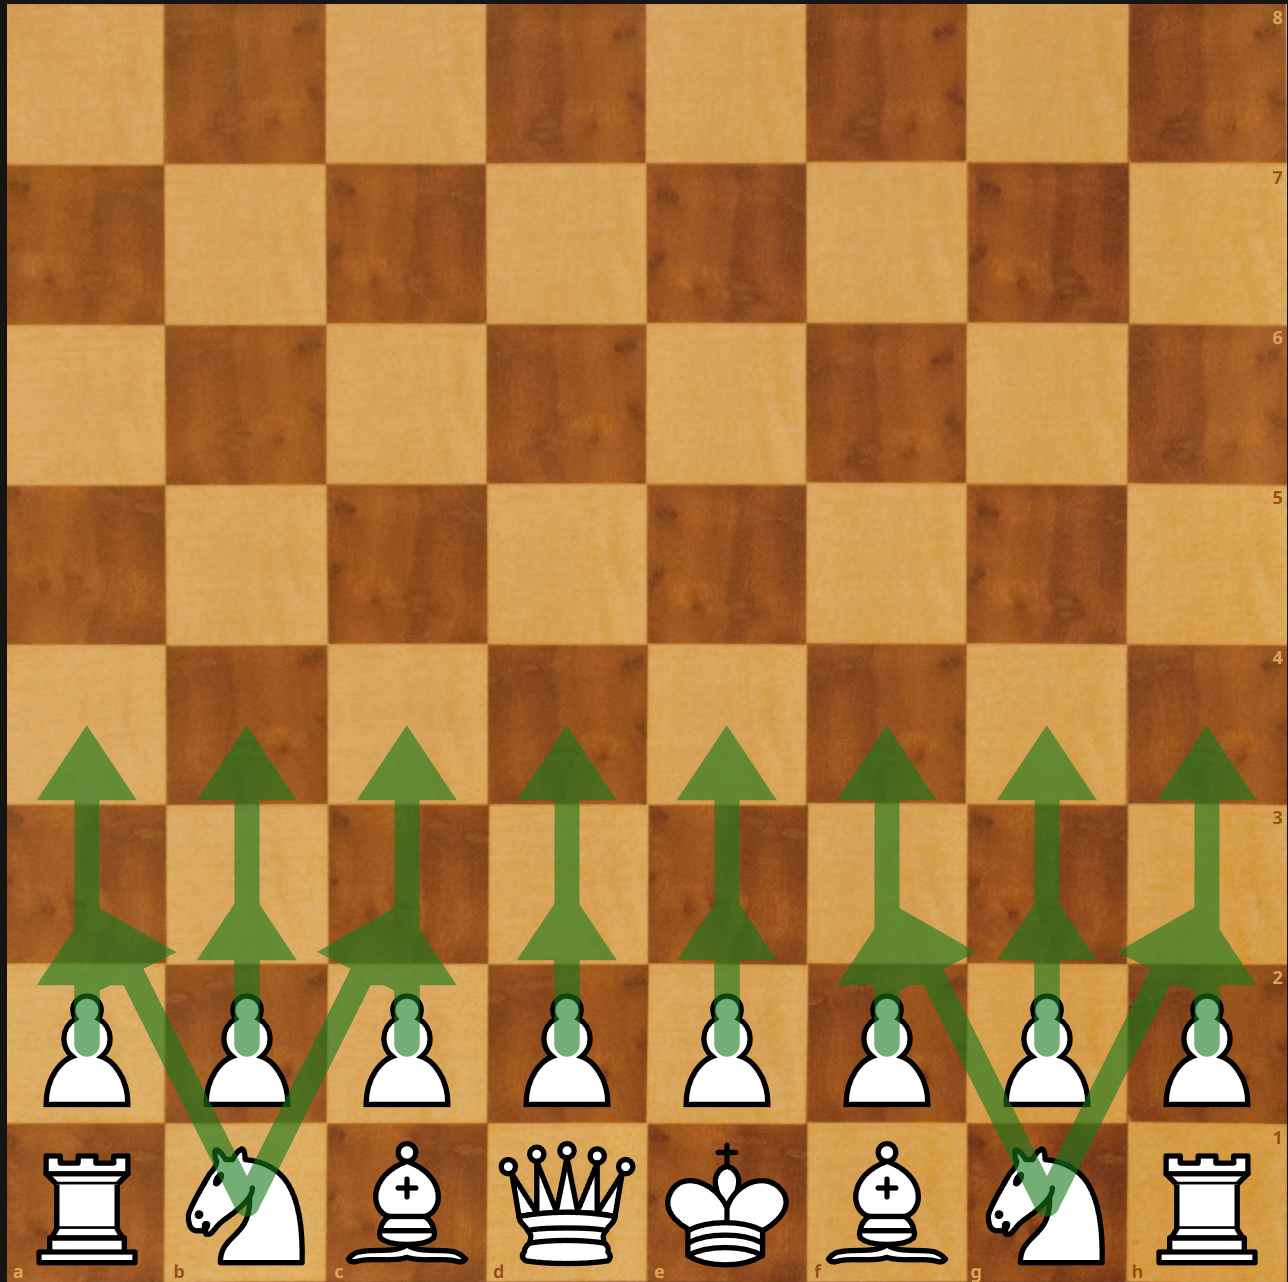
\includegraphics[width=\linewidth/2] {mosse.png}
    \caption{le 20 mosse iniziali possibili per il giocatore bianco ad inizio partita}
    \label{mosse}
\end{figure}






\section{Risultati ottenuti}
È stato ottenuto un motore scacchistico di medio livello che implementa tutte le componenti più importanti, in grado di essere 
capito da un novizio ma che allo stesso tempo funge da ottima base per lo sviluppo di un motore allo stato dell'arte e che riesce a confrontarsi e 
vincere in maniera convincente contro motori famosi per chi si approccia al mondo degli scacchi computazionali come Vice o TSCP; sono anche
stati raccolti dati sull'effetto di queste tecniche, utilizzati per produrre una prova della loro efficacia.



\section{Struttura della tesi}
La tesi è strutturata in 5 capitoli:
\begin{itemize}
\item Il primo funge da introduzione ed illustra a grandi linee il contenuto della tesi. 
\item Nel secondo viene affrontato il processo di progettazione di un motore scacchistico dal punto di vista teorico.
\item Nel terzo vengono illustrati gli effetti pratici delle scelte effettuate nel secondo capitolo.
\item Il quarto è una panoramica sullo stato dell'arte dei motori scacchistici odierni.
\item Il quinto rappresenta uno specchio sui possibili sviluppi di un motore costruito a partire da questa tesi.
\end{itemize}

\chapter{Progettazione e implementazione} %\label{1cap:spinta_laterale}
% [titolo ridotto se non ci dovesse stare] {titolo completo}
%

\begin{citazione}
    In questo capitolo viene mostrato passo passo un procedimento guida alla realizazzione di un motore scacchistico
\end{citazione}

\newpage
\section{Prefazione} %\label{1sec:scopo}
Lo sviluppo di un motore scacchistico è fortemente influenzato dalle scelte progettuali,
una di queste è il linguaggio di programmazione che si vuole utilizzare,
le prestazioni di un motore possono essere fortemente influenzate dalla natura del linguaggio di
programmazione, in particolare l'utilizzo di un linguaggio interpretato e non compilato può impattare
notevolmente sulla velocità con la quale il nostro motore è in grado di elaborare le milioni di
posizioni con le quali dovrà avere a che fare in una singola partita.
Tutti gli esempi di codice all'interno di questa tesi saranno scritti nel linguaggio C, si consiglia
quindi di avere almeno una minima familiarità con tale linguaggio.Si segnalano comunque diversi
tool  per il linguaggio python per chi volesse approcciarsi a questo mondo utilizzando un
linguaggio più beginner friendly  quali:
\begin{itemize}
    \item \textbf{python-chess}: una libreria di python che contiene funzioni di libreria per la rappresentazione
          di scacchiera e pezzi e per la generazione e validazione delle mosse,utile se ci si vuole concentrare
          esclusivamente sulla parte di ricerca e di valutazione  di un motore scacchistico.
    \item \textbf{Sunfish}: un motore scacchistico per principianti scritto nel linguaggio python che
          in sole 111 linee di codice illustra ,in maniera semplificata, l'implementazione della
          gran parte dei concetti  chiave di un motore scacchistico.

\end{itemize}


\section{Rappresentazione della scacchiera e dei pezzi} %\label{1sec:scopo}
Il primo passo dello sviluppo di un motore scacchistico è decidere come si vuole rappresentare
la scacchiera , si tratta di una scelta fondamentale,non solo perché in seguito ci permetterà
di testare le funzioni che andremo a implementare, ma anche perché è nella scacchiera che ,generalmente,
viene conservato lo stato generale della partita.\footnote{per stato di una partita si intendono informazioni come
    informazioni su chi ha diritto di muovere, i permessi di arrocco,lo stato della regola delle 50 mosse etc}
Inoltre il tipo di codifica può influenzare la rapidità
e la facilità col quale possiamo accedere alle informazioni sullo stato corrente dei pezzi
e come vedremo in seguito è in grado di influenzare funzioni come la generazione delle mosse.
Non è raro per motori scacchistici particolarmente complessi l'utilizzo di più tipi di board in base
al tipo di informazione da conservare e all'utilizzo che se ne vuole fare.
Per la rappresentazione di una scacchiera sono chiaramente possibili moltissime scelte, di seguito
verranno illustrate alcune tra le più popolari ed utilizzate.

\subsection{Rappresentazione Pezzocentrica}
Si definisce rappresentazione pezzocentrica, un qualsiasi tipo di rappresentazione della scacchiera che mantiene liste
array o set dei pezzi attualmente presenti sulla scacchiera con annesse le informazioni sulle caselle da essi occupate.
Le rappresentazioni più comuni sono:
\subsubsection{Piece-Lists}
liste o array di ogni pezzo sulla scacchiera,ogni elemento della lista o dell'array associa un pezzo
alla casella che esso occupa .le caratteristiche di ogni pezzo (colore,tipo etc)
possono essere associate all'indice dell'array in cui si trovano o essere presenti in ulteriori array
o liste esterne. \emph{un'implementazione pratica di una Piece-List verrà mostrata in seguito all'interno
    di questo capitolo}

\subsubsection{Bitboards}
Una Bitboard è una struttura dati specifica per i giochi da tavolo,
si tratta in sostanza  di una struttura dati in grado di immagazzinare lo stato di ogni casella della
scacchiera all'interno di una parola \footnote{Una parola è un gruppo di bit di una determinata dimensione che sono gestiti come unità dal set di istruzioni o dall'hardware di un processore} di 64 bit.
Vediamo un esempio pratico, immaginiamo di avere una scacchiera che si trova nello stato di default di inizio
partita:\\
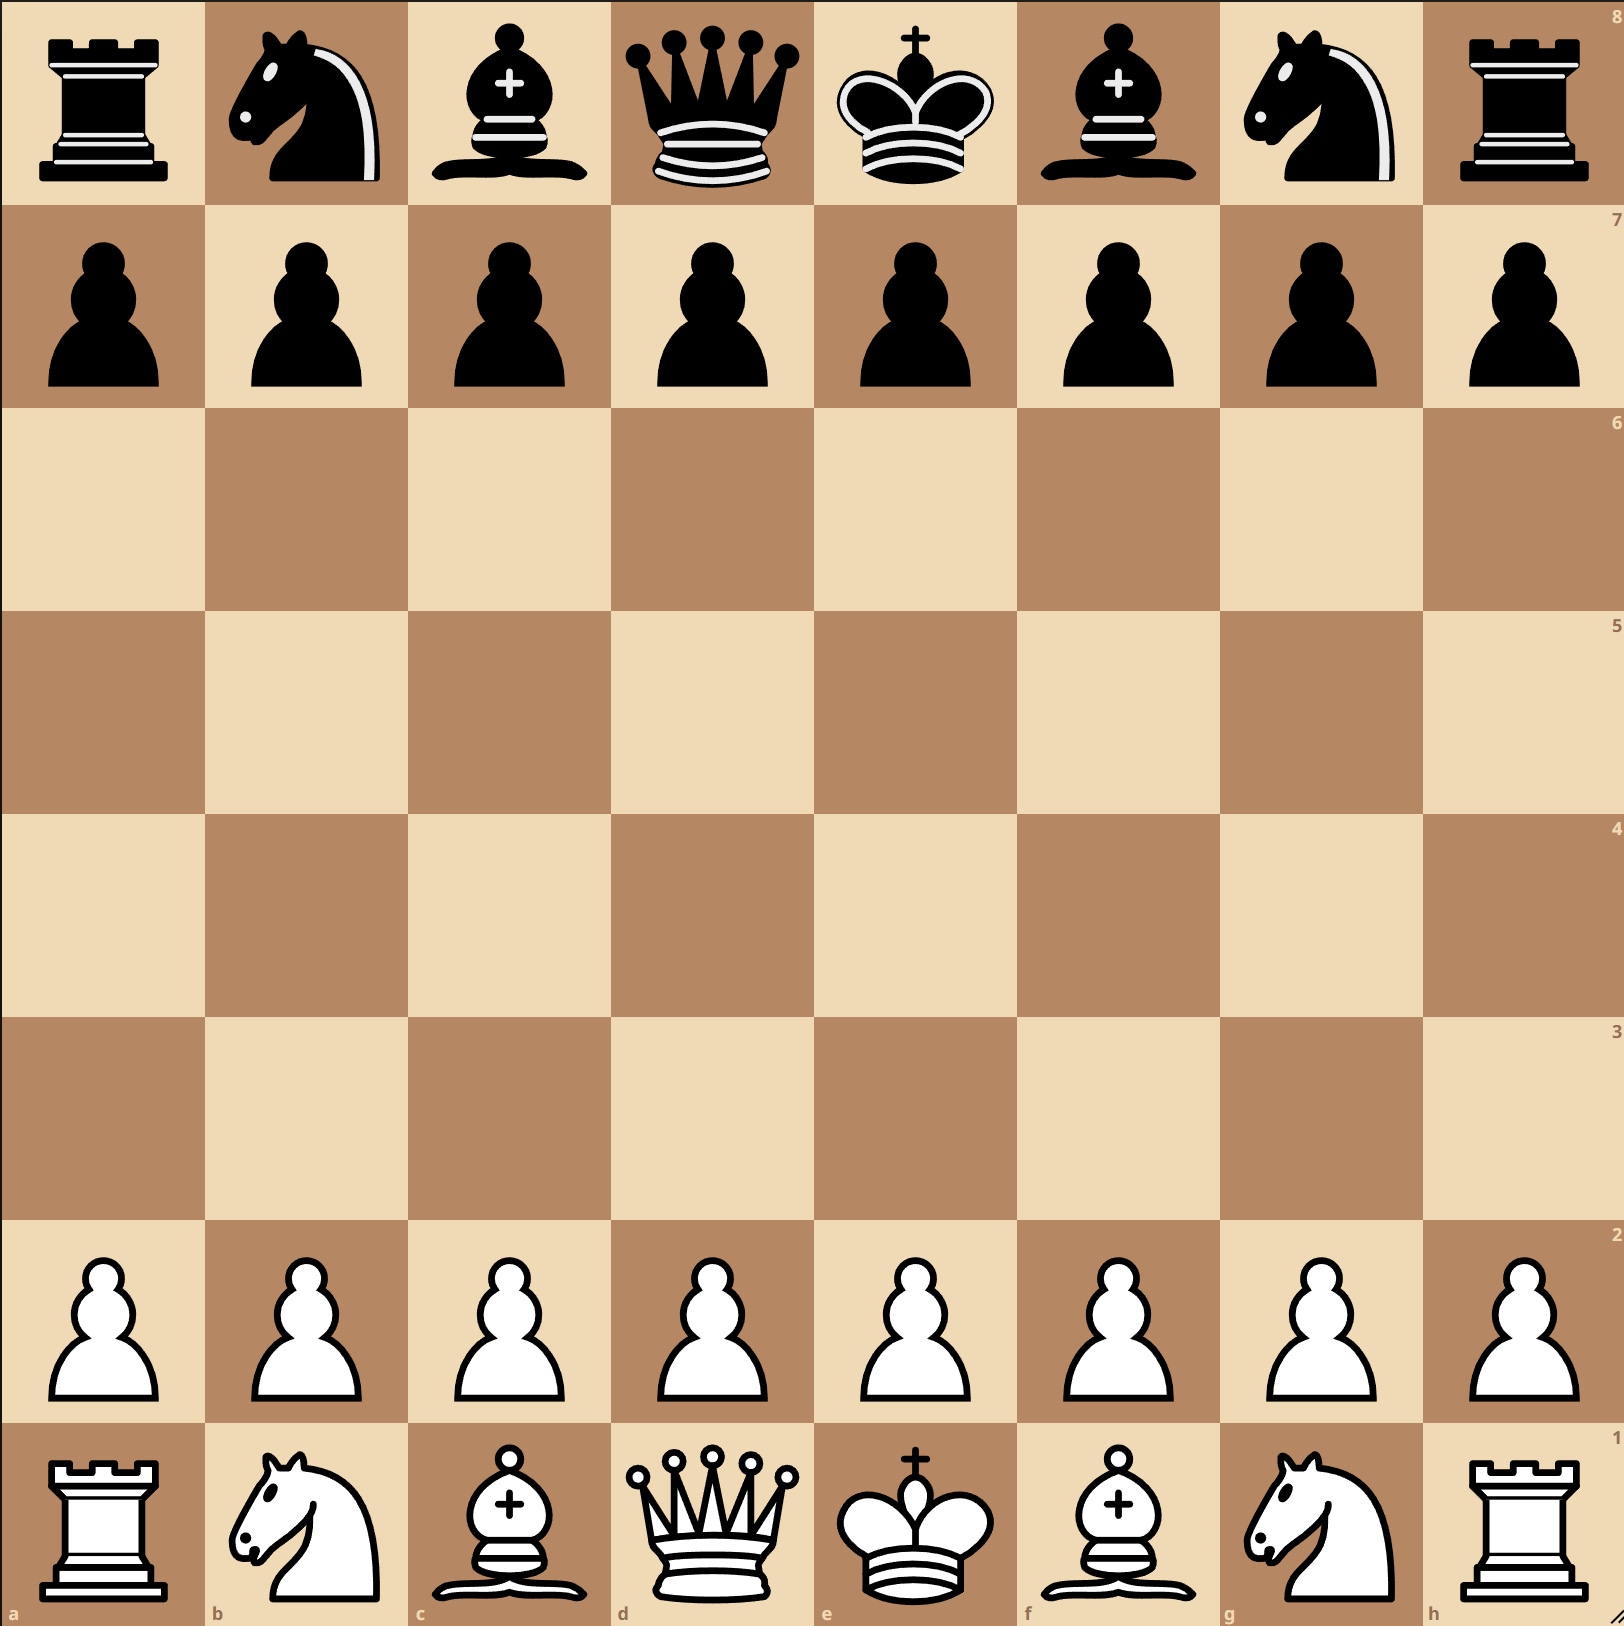
\includegraphics[width=\linewidth] {scacchiera.png}\\
Una bitboard tipica è quella che ci permette di sapere in quali caselle è presente un pedone
nero,per costruirla, operando casella per casella, ci poniamo una domanda "in questa casella
è presente un pedone nero?" se si allora quella casella viene marcata con un 1 , altrimenti viene
marcata con uno 0, il risultato di questa traduzione diventa in questo caso:\\
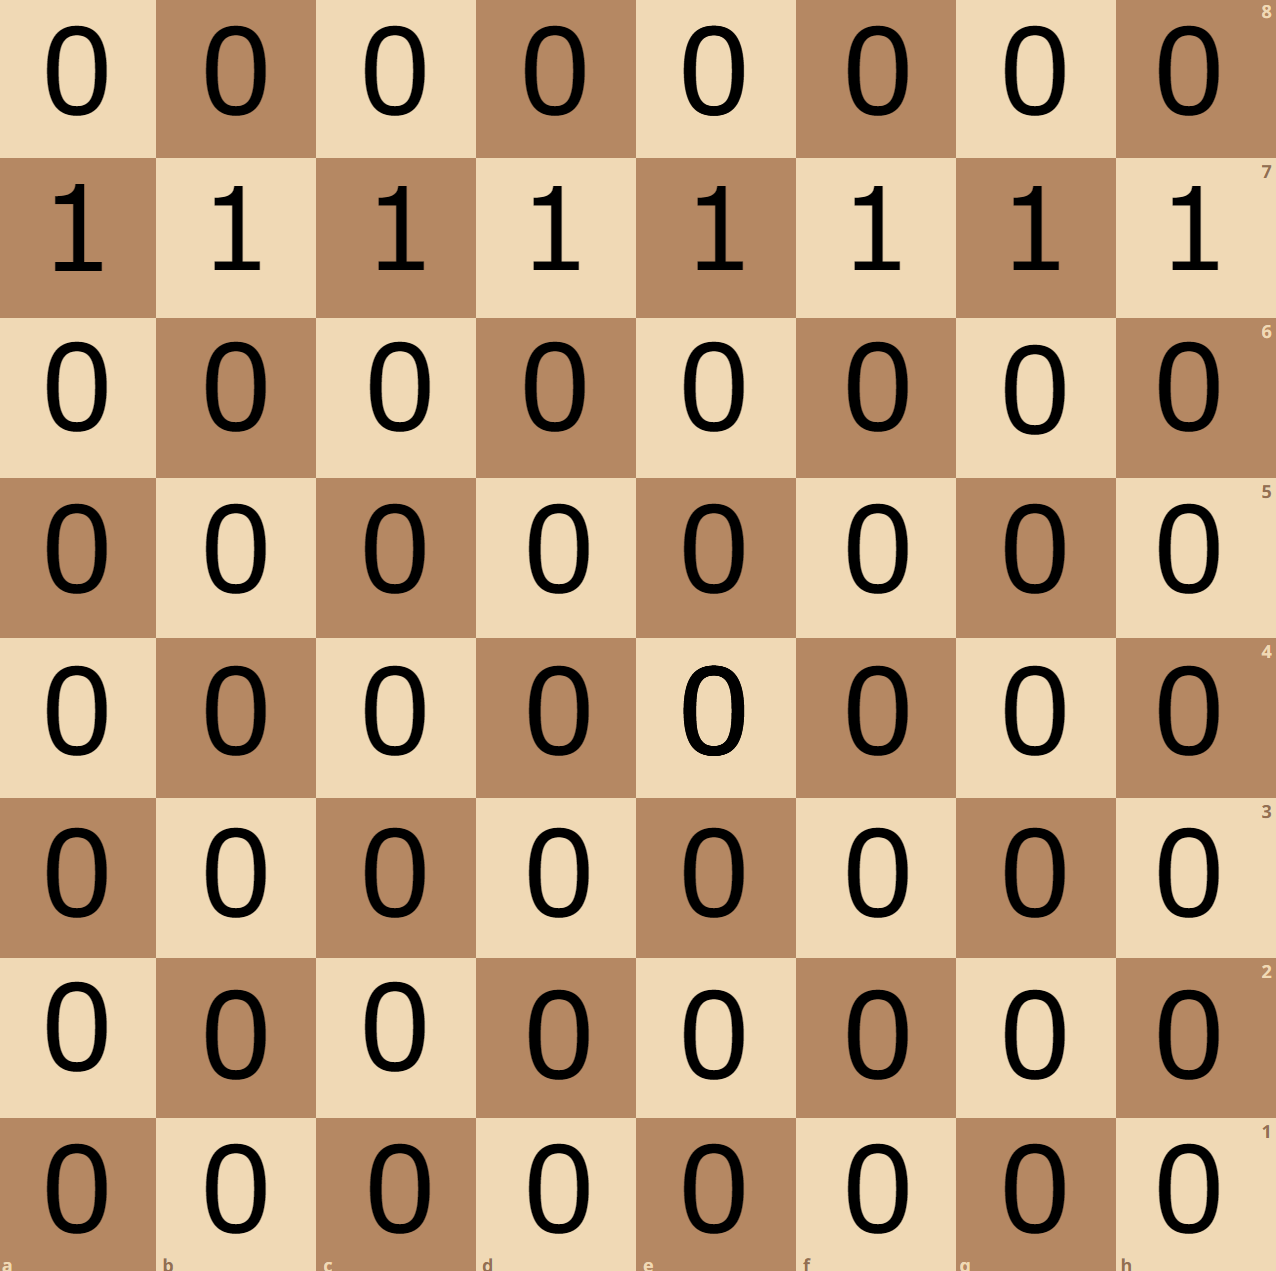
\includegraphics[width=\linewidth] {bitboard.png}\\
La bitboard che codifica questa informazione sarà quindi la parola di 64 bit 00000000 11111111 00000000 00000000 00000000
00000000 00000000 00000000
\subsubsection{Piece-Sets}
rappresentazione con set con un bit per ogni pezzo dentro una parola a 32 bit o 2 parole a 16 bit per ogni lato.
i Piece-sets hanno  delle somiglianze con le bitboards, ma ogni  bit del set non è   direttamente correlato ad una casella,
ma ad un indice  dentro ad una  piece-list. Spesso la bit-position di un  piece-set  implica
, di che tipo e colore il pezzo è. - mentre le  bitboards solitamente mantengono set distinti
per pezzi diversi.
\newpage
\vfill

\begin{figure}
    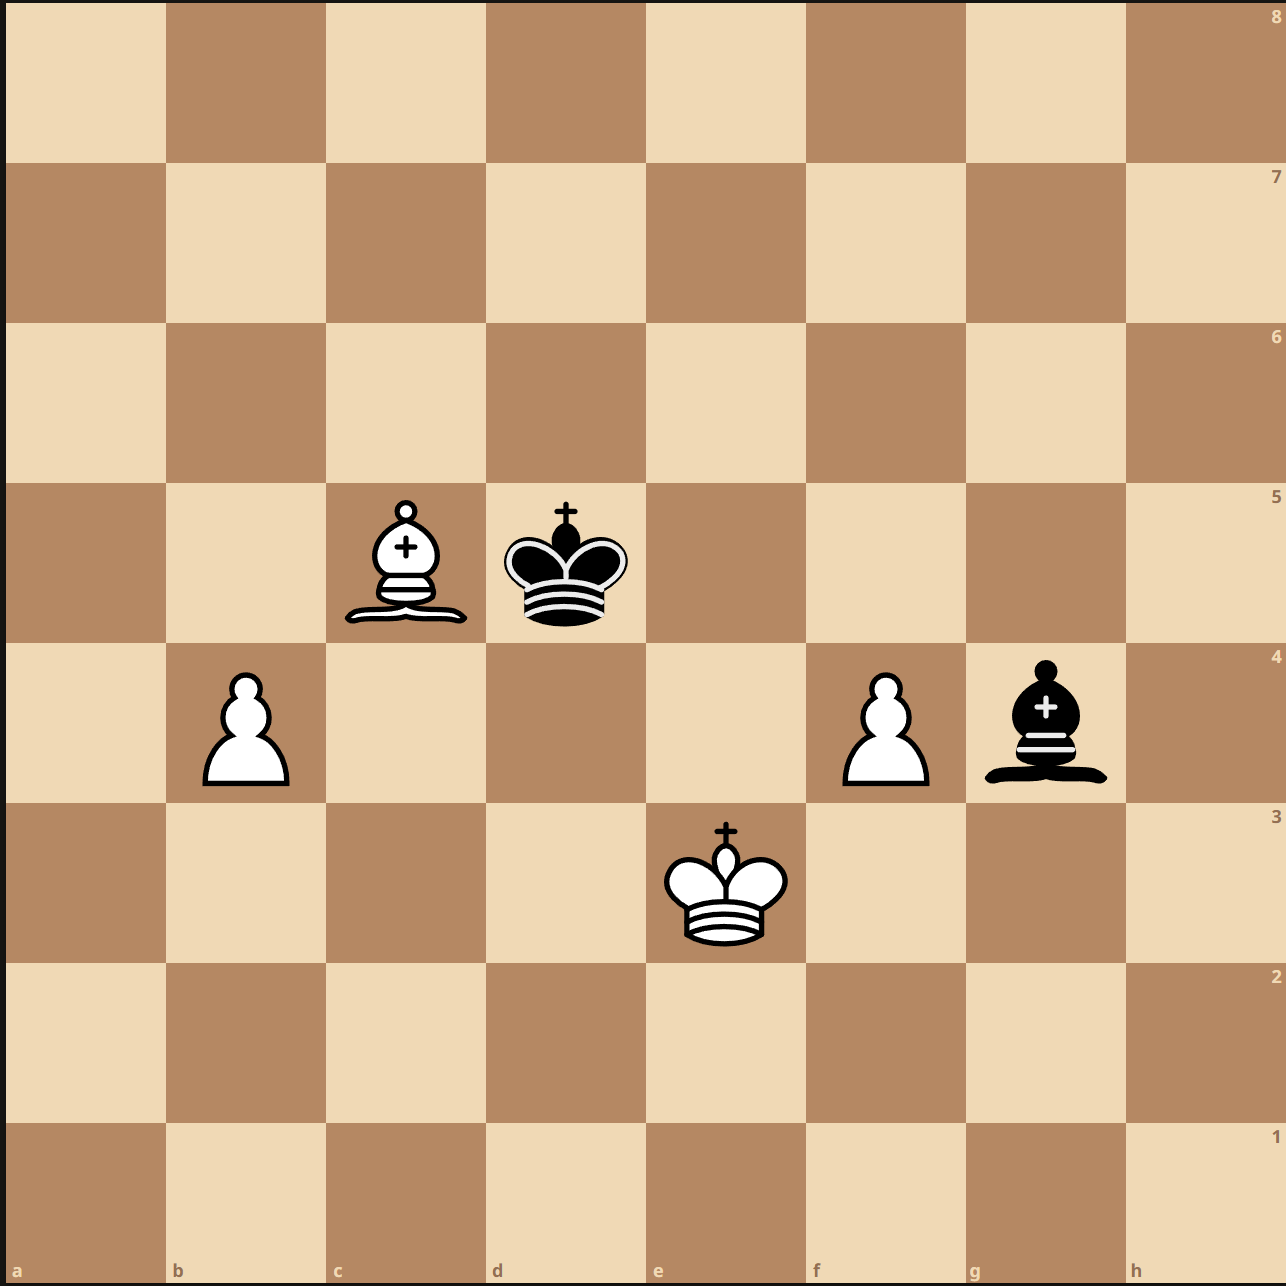
\includegraphics[width=\linewidth]{board.png}
    \caption{Scacchiera nella classica posizione di finale con alfieri di colore opposto }
    \label{board}
\end{figure}

\begin{figure}
    \centering
    
\includegraphics[scale=0.2]{placeholder.png}
    \caption{Rappresentazione set-wise della scacchiera \ref{board} }
\end{figure}

\vfill
\clearpage


\subsection{Rappresentazione Casellocentrica}
La rappresentazione casellocentrica invece mantiene un associazione inversa rispetto a quella pezzocentrica,
per ogni casella conserviamo in memoria se è vuota o occupata da un pezzo in particolare.
La macro-categoria di  rappresentazione più comune è la Mailbox:

\subsubsection{Mailbox}
La rappresentazione Mailbox è una rappresentazione casellocentrica dove la codifica di ogni casella risiede in una struttura dati
che permette l'accesso casuale ,solitamente si utilizza un array con l'indice che codifica dal numero della casella in array monodimensionali
o dalla coppia traversa/colonna\footnote{termini scacchistici per indicare le righe e le colonne della scacchiera} in array bidimensionali.
Il nome deriva dall'associazione di ogni indice al concetto di "indirizzo" di una casella postale.Le implementazioni più famose e
comuni del concetto di Mailbox sono la 8x8 Board, la 10x12 Board e la Vector Attacks.

\subsubsection{8x8 Board}
Una board 8x8 è una rappresentazione pezzocentrica consistente o in un array bidimensionale di bytes o interi, contenenti rappresentazioni codificate
per i pezzi e per la casella vuota, con i due indici ricavati dalla coppia traversa/colonna che identifica la casella sulla scacchiera , 
o più comunemente un array monodimensionale con indici da 0 a 63,uno per ogni casella della scacchiera.
Questo tipo di rappresentazione è usata spesso come rappresentazione ridondante all'interno di programmi che utilizzano bitboards
per individuare se e quali pezzi sono presenti su una casella in maniera efficiente.\\
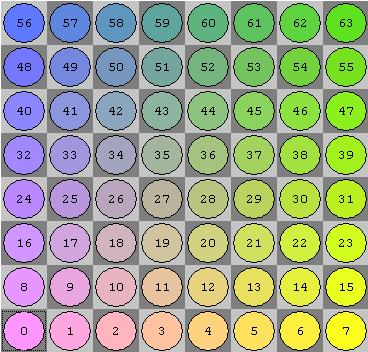
\includegraphics[width=\linewidth]{8x8 board.png}

\subsubsection{10x12 Board}
Una board 10x12  contorna una  board 8x8   con traverse e colonne sentinelle  per individuare  indici off the board while generating moves
using offsets per piece and direction to determine move target squares. Two ranks at the bottom and top are necessary to ensure even knight jumps
from the corners result in valid array indices greater or equal zero and less than 120.

\subsubsection{Vector Attacks}
the application of vectors in the Chebyshev vector space of a chessboard to the problem of chess attacks, including static exchange evaluation (SEE)
, and testing whether moves are pseudo-legal.

\subsubsection{0x88}
a square centric board representation. It uses one nibble for both rank and file each, to index the piece- or empty square codes. While the doubled
array size is negligible, the redundancy of the bit-gaps pays off for several applications. 0x88 is C-syntax and the hexadecimal value of a mask of
bits need to be zero for valid square coordinates (136 decimal, 210 octal, 10001000B).





\section{Move Generation} %\label{1sec:scopo}


\section{Ricerca} %\label{1sec:scopo}

\section{Valutazione} %\label{1sec:scopo}

\section{libro delle aperture,Tablebases} %\label{1sec:scopo}


\chapter{Validazione preliminare} %\label{1cap:spinta_laterale}
% [titolo ridotto se non ci dovesse stare] {titolo completo}
%


\begin{citazione}
In questo capitolo verrà affrontato il problema della validazione di un motore scacchistico,verranno quindi introdotti i concetti fondamentali alla base della valutazione di un motore e saranno forniti 
degli esempi pratici
\end{citazione}

\newpage
\section*{Validazione preliminare}
Essendo un motore scacchistico un progetto che per sua stessa natura va affrontato con un processo di integrazione continua si rende necessario avere un metodo 
per poter calcolare la nuova forza stimata del motore  ad ogni singolo cambiamento  delle funzioni di ricerca e di valutazione,per assicurarci che i cambiamenti apportati non abbiano reso il motore più debole\footnote{Questo tipo di test è anche detto test di regressione}.
Prima di parlare di "perdere" o "acquisire" forza, è bene introdurre come si quantifica e cosa rappresenta la forza di un motore, il sistema di rappresentazione è mutuato dal sistema utilizzato per classificare i 
giocatori di scacchi da parte delle federazioni scacchistiche, ed è un sistema che prende il nome di ELO, essendo gli scacchi un gioco in cui  rendimento di un giocatore non può essere misurato in maniera assoluta,
ma può solo essere dedotto dai risultati i punteggi hanno significato solo relativamente ai punteggi degli avversari: 
sia la media sia l'intervallo dei punteggi possono essere scelti arbitrariamente. Elo suggerì una scala per cui una differenza di 200 punti significa che il giocatore ha un punteggio atteso di 0,75.
Il punteggio atteso di un giocatore è dato dalla probabilità di vincere, più la metà della probabilità di pareggiare. Quindi un punteggio atteso di 0,75 può rappresentare un 75\% di possibilità di vittoria, 
25\% di sconfitta e 0\% di pareggio, o all'altro estremo 50\% di vittoria, 0\% di sconfitta e 50\% di pareggio.

Se il giocatore A ha una forza reale RA e il giocatore B una forza reale RB, la formula esatta (usando la curva logistica) per calcolare il punteggio atteso del giocatore A è:

\begin{equation}  E_{A}={\frac{{1}}{{1+10^\frac{{{RB} - {RA}}}{{400}}}}} \end{equation}
Similarmente, il punteggio atteso del giocatore B è:
\begin{equation}  E_{B}={\frac{{1}}{{1+10^\frac{{{RA} - {RB}}}{{400}}}}} \end{equation}

Si noti che {\begin{equation}E_{A} +  E_{B}=1 \end{equation}

In pratica, siccome la forza reale di un giocatore è sconosciuta, i punteggi attesi sono calcolati utilizzando i punteggi effettivi dei giocatori. Quando i risultati di un giocatore eccedono il punteggio atteso,
il sistema ELO considera il fatto come evidenza che il punteggio del giocatore è troppo basso: perciò deve essere aggiustato verso l'alto. Se invece i risultati restano sotto il punteggio atteso, 
il punteggio del giocatore viene aggiustato verso il basso. L'idea originale di Elo  ,ancora largamente usata , è quella di un semplice aggiustamento lineare, proporzionale a quanto il giocatore sia stato
sopra o sotto il punteggio atteso. 
Supponendo che il giocatore A abbia un punteggio atteso di ${E_{A}}$ punti, ma abbia ottenuto ${S_{A}}$ punti. La formula per aggiornare il suo punteggio è:

\begin{equation} R_{A}' =R_{A}+K(S_{A}-E_{A})\end{equation}

L'aggiornamento può essere effettuato dopo ogni partita, dopo ogni torneo, o dopo ogni periodo prestabilito. Un esempio può aiutare a comprendere. Supponiamo che il giocatore A abbia un punteggio di 1613, 
e giochi in un torneo con cinque partite. Perde contro un giocatore quotato 1609, pareggia con un giocatore che ha 1477 punti, sconfigge un giocatore con 1388 punti, e uno con 1586, e infine perde con un giocatore 
che ha 1720 punti. Il suo punteggio è $ {(0+0,5+1+1+0)=2,5}$. il suo punteggio atteso, calcolato secondo la formula sopra esposta, avrebbe dovuto essere 
$ (0,506+0,686+0,785+0,539+0,351)=2,867 $. Quindi il suo nuovo punteggio è (1613+32(2,5-2,867))=1601} \cite{itwiki:125247032}.

Come detto precedentemente cosi come per i giocatori umani anche per i motori viene utilizzato il concetto di ELO per la misura delle prestazioni,ci sono però delle differenze pratiche sostanziali,in primis,
a differenza di un giocatore umano , dove " l'hardware" è immutabile, la forza di un motore scacchistico dipende anche dalla potenza di calcolo della macchina sul quale gira, ed in secundis l'elo può dipendere 
da fattori esterni come la gestione del tempo che si ha a disposizione per una mossa,questo è un problema che si applica anche ai giocatori umani ma che fa intrinsecamente parte del loro punteggio in quanto 
un giocatore umano ha libertà di gestire come vuole il proprio tempo, a differenza di un motore scacchistico dove ,soprattutto in motori più basilari, è possibile che il tempo sia gestito in maniera statica.
Per ovviare a questo problematiche ed ottenere una misura di elo significativa è importante uniformare il più possibile la piattaforma sulla quale si effettuano le prove e valutare con attenzione il time control utilizzato.

\begin{figure}[h]
    \centering
    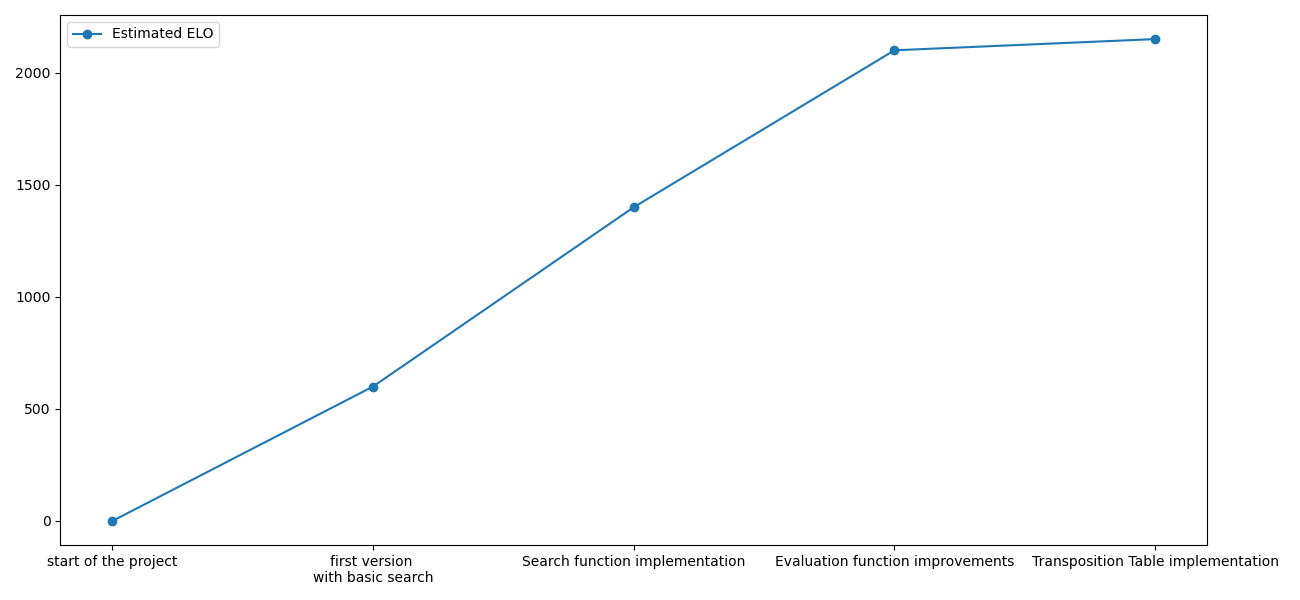
\includegraphics[width=\textwidth]{myplot.png}
    \caption{Valore ELO del motore sviluppato parallelamente a questa tesi ad ogni milestone di sviluppo}
\end{figure}

Oltre al punteggio ELO esistono altre metriche che possono essere utilizzate per analizzare singolarmente alcune delle componenti che compongono un motore,
per la generazione delle mosse abbiamo già visto nel paragrafo \ref{move generation} che è possibile utilizzare la funzione di Perft per valutare le prestazioni di un generatore di mosse,ed essendo la generazione
delle mosse un concetto molto semplice, possiamo seguire un euristica basilare: "più nodi vengono generati al secondo migliore è il generatore",valutare le parti 
di ricerca non è invece altrettanto facile,se è vero che abbiamo un'idea di fondo alla base dell'ottimizzazione della nostra ricerca,ossia "meno nodi vengono esplorati migliore è la funzione di ricerca", è anche vero 
che questo concetto, a differenza di quello della generazione delle mosse, è sottoposto ad ulteriori clausole,vogliamo si che il nostro algoritmo di ricerca esplori meno nodi possibili, ma vogliamo anche che la qualità
delle scelte possibili venga preservata,un numero minore di nodi esplorati quindi, è positivo solo se la forza giocante del nostro motore non diminuisce (o ancor meglio se aumenta), ciò nonostante il variare del numero dei nodi 
può darci un'idea sulla bontà del trade-off ELO/tempo di calcolo necessario ed in generale indicarci se l'approccio che stiamo seguendo meriti o meno ulteriori approfondimenti.
\begin{table}[h]
\begin{center}
    \begin{tabular}{|c|c|c|c|c|} 
     \hline
     Depth & Total Nodes  & $\alpha\beta$ & CE2BIT & Vice 1.1 \\ [0.5ex] 
     \hline
     1 & 20  & 21 & 27 & 21 \\ 
     \hline
     2 & 400  &  231 & 313 & 89\\
     \hline
     3 & 8902  &  3346 & 654 & 694 \\
     \hline
     4 & 197281  & 18081 &  3407 & 4000 \\
     \hline
     5 & 4865609  & 138712 & 4624 & 11000 \\ 
     \hline
     6 & 119060324  & 774756 & 32490 & 61000\\
     \hline
    \end{tabular}
    \caption{Confronto tra i numeri esplorati da un semplice algoritmo di ricerca alfa-beta e quelli esplorati da diversi motori scacchistici} \label{tab:sometab}
    \end{center}
\end{table}



\chapter{Stato dell'arte per Algoritmi di intelligenza artificiale e motori scacchistici  per il gioco degli scacchi} %\label{1cap:spinta_laterale}
% [titolo ridotto se non ci dovesse stare] {titolo completo}
%

\begin{citazione}
Questo capitolo illustra lo stato dell'arte e i lavori presenti in letteratura sui motori scacchistici
\end{citazione}

\newpage


\section{Stockfish pre rete neurale }
Prima della rivoluzione dei motori scacchistici favoreggiata dall'introduzione di reti neurali nel processo di valutazione di una posizione, che vedremo in seguito,lo stato dell'arte era rappresentato
da una decina di motori con funzioni di valutazione HCE,tra questi è difficile trovare un rappresentante migliore di Stockfish, uno dei motori scacchistici più vincenti di sempre e frutto di un progetto
open source che va ormai avanti da decenni.
\subsection{Struttura interna}
Per la rappresentazione della scacchiera Stockfish non offre sorprese particolari,utilizza un misto di bitboard e board 8x8 per la rappresentazione dei pezzi ed opta per l'utilizzo di bitboard pext
o magiche per la generazione delle mosse.\\La ricerca nelle sue basi è una ricerca di tipo alfa-beta con approfondimento iterativo come già visto in precedenza,vi è anche la presenza di quelle 
aggiunte alla ricerca minimax che in questo campo risultano essere fondamentali, come una tabella di trasposizione e varie euristiche di ordinamento della mossa.\\La vera grande differenza
tra Stockfish ed un motore hobbystico per quanto riguarda la ricerca è l'implementazione di un algoritmo di ricerca multi-thread,si tratta di una versione dell'algoritmo molto complessa in quanto deve
gestire tutti i problemi classici della concorrenza ed in più assicurarsi che il lavoro parallelo dei thread abbia un effetto costruttivo e non distruttivo, in particolare Stockfish implementa l'algoritmo di 
ricerca parallelo chiamato Lazy SMP, nel quale vengono fatte partire diverse ricerche (una per thread) a partire dallo stesso nodo sorgente ma con differenti variabili di ricerca (profondità massime diverse, pesi 
diversi per l'ordinamento delle mosse o per la potatura) ed i risultati vengono conservati in una tabella hash comune a tutte le istanze di ricerca, che possono quindi utilizzare i risultati delle altre per 
auto-guidarsi.Infine, per quanto riguarda la parte di valutazione, ossia quella più complessa e delicata, va detto che non esiste un modo per descrivere brevemente le sottili ed intricate scelte all'interno 
della funzione, in particolare per quanto riguarda i pesi utilizzati dalla funzione obbiettivo, ci basti sapere che a questo punto della storia (pre fine 2017) Stockfish è mosso da una funzione di valutazione 
di tipo HCE, che coinvolge diverse euristiche di tipo scacchistico e centinaia di pesi calibrati a mano dopo milioni e milioni di test di regressione.


\section{AlphaZero}
Alla fine dell'anno 2017 un controverso paper\cite{DBLP:journals/corr/abs-1712-01815} da parte del team di Google DeepMind, apre un nuovo spiraglio di possibilità nel mondo degli scacchi computazionali,
in questo paper infatti viene presentato un motore chiamato AlphaZero, sprovvisto di una funzione di valutazione HCE, fin ora standard praticamente unico del mondo scacchistico, questo motore,complice anche l'enorme 
potenza dei cluster di calcolatori di google, fu un grado di partire dalle sole basi del gioco degli scacchi,senza nessuna conoscenza posizionale fornita esternamente, ed in 4 ore auto-migliorarsi al punto 
da competere e riuscire a vincere in maniera convincente contro la versione di Stockfish dell'anno precedente ma con un approccio da parte del team di ricerca non esente da critiche\cite{chess.com}.



\section{Stockfish-NNUE e LCZero}
Nonostante le critiche ed i dubbi sulla performance di AlphaZero, gli appassionati di scacchi computazionali non rimasero impassibili davanti ai meriti di un approccio orientato alle reti neurali,
il 6 agosto del 2020, un anno e mezzo dopo la pubblicazione definitiva dell'articolo su AlphaZero da parte di DeepMind e dopo un anno di lavoro, viene ufficialmente introdotta ,all'interno della repo di Stockfish,NNUE.
\\NNUE, acronimo di "Effeciently Upgradable Neural Network" scritto da sinistra a destra, è una rete neurale per la valutazione di posizioni shogi, alle quali assegna un punteggio
utilizzato poi in fase di potatura, adattata per operare sugli scacchi ed essere integrata in Stockfish.
In questa nuova versione Stockfish, chiamato da questo momento in poi anche Stockfish+NNUE, mantiene le caratteristiche principali che contraddistinguono la sua versione precedente, e la valutazione NNUE viene
utilizzata in tutte le posizioni materialmente bilanciate.In totale il guadagno di Stockfish dopo il passaggio a NNUE è stato stimato nel range di 80-100 punti ELO.


\chapter{Conclusioni e Sviluppi Futuri} %\label{1cap:spinta_laterale}
% [titolo ridotto se non ci dovesse stare] {titolo completo}
%


\begin{citazione}
	BREVE SPIEGAZIONE CONTENUTO CAPITOLO
\end{citazione}

\newpage

%\part{Impatto ambientale}

\backmatter
%*******************************************************
% Bibliografia
%*******************************************************
\cleardoublepage
\phantomsection
\addcontentsline{toc}{chapter}{\bibname}
\nocite{*}
\bibliographystyle{abbrvnat.bst}
\bibliography{bibliografia}
%


\phantomsection
\chapter{Ringraziamenti}
\markboth{Ringraziamenti}{}
% [titolo ridotto se non ci dovesse stare] {titolo completo}
INSERIRE RINGRAZIAMENTI QUI 
\end{document}
